\documentclass[12pt, a4paper]{article}
\usepackage{../../../myconfig}

\begin{document}

\titlebox{Chủ đề: Oxyz}{Vecto và các phép toán vecto \\ trong không gian}{Oxyz}

% --- CÂU 1 ---
\questionLinesManual{5}{1}{Cho tứ diện \(ABCD\). Mệnh đề nào dưới đây là mệnh đề đúng?}{%
    \begin{tasks}(2)
        \task \(\vec{BC} + \vec{AB} = \vec{DA} - \vec{DC}\)
        \task \(\vec{AC} - \vec{AD} = \vec{BD} - \vec{BC}\)
        \task \(\vec{AB} - \vec{AC} = \vec{DB} - \vec{DC}\)
        \task \(\vec{AB} - \vec{AD} = \vec{CD} + \vec{BC}\)
    \end{tasks}
}

% --- CÂU 2 ---
\questionLinesManual{5}{2}{Cho hình hộp \(ABCD.A'B'C'D'\). Chọn đẳng thức vectơ đúng:}{%
    \begin{tasks}(2)
        \task \(\vec{AC'} = \vec{AB} + \vec{AB'} + \vec{AD}\)
        \task \(\vec{DB'} = \vec{DA} + \vec{DD'} + \vec{DC}\)
        \task \(\vec{AC'} = \vec{AC} + \vec{AB} + \vec{AD}\)
        \task \(\vec{DB} = \vec{DA} + \vec{DD'} + \vec{DC}\)
    \end{tasks}
}

% --- CÂU 3 ---
\questionLinesManual{5}{3}{Cho hình hộp \(ABCD.A'B'C'D'\). Biểu thức nào sau đây đúng:}{%
    \begin{tasks}(2)
        \task \(\vec{A'D} = \vec{A'B'} + \vec{A'C'}\)
        \task \(\vec{AB'} = \vec{AB} + \vec{AA'} + \vec{AD}\)
        \task \(\vec{AC'} = \vec{AB} + \vec{AA'} + \vec{AD}\)
        \task \(\vec{AD'} = \vec{AB} + \vec{AD} + \vec{AC'}\)
    \end{tasks}
}

% --- CÂU 4 ---
\questionLinesManual{5}{4}{Cho tứ diện \(ABCD\). Gọi \(M, N\) lần lượt là trung điểm của \(AD\) và \(BC\). Khẳng định nào sau đây \textbf{sai}?}{%
    \begin{tasks}(2)
        \task \(\vec{AB} + \vec{CD} = \vec{CB} + \vec{AD}\)
        \task \(2\vec{MN} = \vec{AB} + \vec{DC}\)
        \task \(\vec{AD} + 2\vec{MN} = \vec{AB} + \vec{AC}\)
        \task \(2\vec{MN} = \vec{AB} + \vec{AC} + \vec{AD}\)
    \end{tasks}
}

% --- CÂU 5 ---
\questionLinesManual{5}{5}{Cho hình chóp \(S.ABCD\) có đáy \(ABCD\) là hình bình hành. Khẳng định nào sau đây \textbf{đúng}?}{%
    \begin{tasks}(2)
        \task \(\vec{SA} + \vec{SD} = \vec{SB} + \vec{SC}\)
        \task \(\vec{SA} + \vec{SB} + \vec{SC} + \vec{SD} = \vec{0}\)
        \task \(\vec{SA} + \vec{SC} = \vec{SB} + \vec{SD}\)
        \task \(\vec{SA} + \vec{SB} = \vec{SC} + \vec{SD}\)
    \end{tasks}
}

% --- CÂU 6 ---
\questionLinesManual{5}{6}{Cho tứ diện \(ABCD\). Gọi \(I, J\) lần lượt là trung điểm của \(AB\) và \(CD\), \(G\) là trung điểm của \(IJ\). Cho các đẳng thức sau, đẳng thức nào đúng?}{%
    \begin{tasks}(2)
        \task \(\vec{GA} + \vec{GB} + \vec{GC} + \vec{GD} = \vec{0}\)
        \task \(\vec{GA} + \vec{GB} + \vec{GC} + \vec{GD} = 2\vec{IJ}\)
        \task \(\vec{GA} + \vec{GB} + \vec{GC} + \vec{GD} = \vec{JI}\)
        \task \(\vec{GA} + \vec{GB} + \vec{GC} + \vec{GD} = -2\vec{JI}\)
    \end{tasks}
}

% --- CÂU 7 ---
\questionLinesManual{5}{7}{Cho hình lăng trụ tam giác \(ABCA'B'C'\). Đặt \(\vec{AA'} = \vec{a}, \vec{AB} = \vec{b}, \vec{AC} = \vec{c}, \vec{BC} = \vec{d}\). Trong các biểu thức vectơ sau đây, biểu thức nào đúng.}{%
    \begin{tasks}(4)
        \task \(\vec{a} + \vec{b} + \vec{c} = \vec{d}\)
        \task \(\vec{a} = \vec{b} + \vec{c}\)
        \task \(\vec{a} + \vec{b} + \vec{c} + \vec{d} = \vec{0}\)
        \task \(\vec{b} - \vec{c} + \vec{d} = \vec{0}\)
    \end{tasks}
}

% --- CÂU 8 ---
\questionLinesManual{5}{8}{Trong không gian cho điểm \(O\) và bốn điểm \(A, B, C, D\) không thẳng hàng. Điều kiện cần và đủ để \(A, B, C, D\) tạo thành hình bình hành là:}{%
    \begin{tasks}(2)
        \task \(\vec{OA} + \vec{OB} + \vec{OC} + \vec{OD} = \vec{0}\)
        \task \(\vec{OA} + \vec{OC} = \vec{OB} + \vec{OD}\)
        \task \(\vec{OA} + \dfrac{1}{2}\vec{OB} = \vec{OC} + \dfrac{1}{2}\vec{OD}\)
        \task \(\vec{OA} + \dfrac{1}{2}\vec{OC} = \vec{OB} + \dfrac{1}{2}\vec{OD}\)
    \end{tasks}
}

% --- CÂU 9 ---
\questionLinesManual{5}{9}{Cho hình hộp chữ nhật \(ABCD.A'B'C'D'\). Khi đó, vectơ bằng vectơ \(\vec{AB}\) là vectơ nào dưới đây?}{%
    \begin{tasks}(4)
        \task \(\vec{D'C'}\)
        \task \(\vec{BA}\)
        \task \(\vec{CD}\)
        \task \(\vec{B'A'}\)
    \end{tasks}
}

% --- CÂU 10 ---
\questionLinesManual{4}{10}{Cho hình lập phương \(ABCD.A_1B_1C_1D_1\). Gọi \(O\) là tâm của hình lập phương. Chọn đẳng thức đúng?}{%
    \begin{tasks}(2)
        \task \(\vec{AO} = \dfrac{1}{3}\left( \vec{AB} + \vec{AD} + \vec{AA_1} \right)\)
        \task \(\vec{AO} = \dfrac{1}{2}\left( \vec{AB} + \vec{AD} + \vec{AA_1} \right)\)
        \task \(\vec{AO} = \dfrac{1}{4}\left( \vec{AB} + \vec{AD} + \vec{AA_1} \right)\)
        \task \(\vec{AO} = \dfrac{2}{3}\left( \vec{AB} + \vec{AD} + \vec{AA_1} \right)\)
    \end{tasks}
}

% --- CÂU 11 ---
\questionLinesManual{4}{11}{Cho tứ diện \(ABCD\). Gọi \(G\) là trọng tâm tam giác \(ABC\). Tìm giá trị của \(k\) thích hợp điền vào đẳng thức vectơ: \(\vec{DA} + \vec{DB} + \vec{DC} = k\vec{DG}\)}{%
    \begin{tasks}(4)
        \task \(k = 2\)
        \task \(k = 3\)
        \task \(k = \dfrac{1}{2}\)
        \task \(k = \dfrac{1}{3}\)
    \end{tasks}
}

% --- CÂU 12 ---
\questionLinesManual{5}{12}{Cho tứ diện \(ABCD\). Gọi \(P, Q\) là trung điểm của \(AB\) và \(CD\). Chọn khẳng định đúng?}{%
    \begin{tasks}(2)
        \task \(\vec{PQ} = \dfrac{1}{2}\left( \vec{BC} + \vec{AD} \right)\)
        \task \(\vec{PQ} = \dfrac{1}{2}\left( \vec{BC} - \vec{AD} \right)\)
        \task \(\vec{PQ} = \vec{BC} + \vec{AD}\)
        \task \(\vec{PQ} = \dfrac{1}{4}\left( \vec{BC} + \vec{AD} \right)\)
    \end{tasks}
}

% --- CÂU 13 ---
\questionLinesManual{5}{13}{Cho tứ diện \(ABCD\). Gọi \(M\) và \(N\) lần lượt là trung điểm của \(AB\) và \(CD\). Tìm giá trị của \(k\) thích hợp điền vào đẳng thức vectơ: \(\vec{MN} = k\left( \vec{AC} + \vec{BD} \right)\)}{%
    \begin{tasks}(4)
        \task \(k = 2\)
        \task \(k = \dfrac{1}{2}\)
        \task \(k = \dfrac{1}{3}\)
        \task \(k = 3\)
    \end{tasks}
}

% --- CÂU 14 ---
\questionLinesManual{5}{14}{Cho hình hộp \(ABCD.A_1B_1C_1D_1\). Trong các khẳng định sau, khẳng định nào \textbf{sai}?}{%
    \begin{tasks}(2)
        \task \(\vec{C_1A_1} + \vec{A_1C} = \vec{CC_1}\)
        \task \(\vec{AC_1} + \vec{CA_1} + 2\vec{C_1C} = \vec{0}\)
        \task \(\vec{AC_1} + \vec{A_1C} = \vec{AA_1}\)
        \task \(\vec{AC_1} + \vec{A_1C} = 2\vec{AC}\)
    \end{tasks}
}

% --- CÂU 15 ---
\questionLinesManual{5}{15}{Cho tứ diện \(ABCD\) và \(I\) là trọng tâm tam giác \(ABC\). Đẳng thức đúng là.}{%
    \begin{tasks}(2)
        \task \(\vec{SI} = \vec{SA} + \vec{SB} + \vec{SC}\)
        \task \(\vec{SI} = 3\left( \vec{SA} - \vec{SB} + \vec{SC} \right)\)
        \task \(\vec{SI} = \dfrac{1}{3}\vec{SA} + \dfrac{1}{3}\vec{SB} + \dfrac{1}{3}\vec{SC}\)
        \task \(6\vec{SI} = \vec{SA} + \vec{SB} + \vec{SC}\)
    \end{tasks}
}

% --- CÂU 16 ---
\questionLinesManual{5}{16}{Cho hình lập phương \(ABCDEFGH\), thực hiện phép toán: \(\vec{x} = \vec{CB} + \vec{CD} + \vec{CG}\)}{%
    \begin{tasks}(4)
        \task \(\vec{x} = \vec{CE}\)
        \task \(\vec{x} = \vec{CH}\)
        \task \(\vec{x} = \vec{EC}\)
        \task \(\vec{x} = \vec{GE}\)
    \end{tasks}
}

% --- CÂU 17 ---
\questionLinesManual{5}{17}{Cho hình chóp \(S.ABCD\) có đáy là hình bình hành tâm \(O\). Gọi \(G\) là điểm thỏa mãn: \(\vec{GS} + \vec{GA} + \vec{GB} + \vec{GC} + \vec{GD} = \vec{0}\). Trong các khẳng định sau, khẳng định nào đúng?}{%
    \begin{tasks}(2)
        \task \(G, S\) không thẳng hàng.
        \task \(\vec{GS} = 4\vec{OG}\)
        \task \(\vec{GS} = 5\vec{OG}\)
        \task \(\vec{GS} = 3\vec{OG}\)
    \end{tasks}
}

% --- CÂU 18 ---
\questionLinesManual{5}{18}{Cho hình hộp \(ABCD.A'B'C'D'\). Tìm giá trị của \(k\) thích hợp điền vào đẳng thức vectơ: \(\vec{BD} - \vec{D'D} - \vec{B'D'} = k\vec{BB'}\)}{%
    \begin{tasks}(4)
        \task \(k = 4\)
        \task \(k = 1\)
        \task \(k = 0\)
        \task \(k = 2\)
    \end{tasks}
}

% --- CÂU 19 ---
\questionLinesManual{5}{19}{Cho hình lập phương \(ABCD.A_1B_1C_1D_1\) (Tham khảo hình vẽ bên).
\begin{center}
    \begin{tikzpicture}[scale=1.2]
    % Định nghĩa tọa độ các đỉnh đáy dưới ABCD
    \coordinate (A) at (0, 0);
    \coordinate (B) at (-1.2, -0.8);
    \coordinate (C) at (1.3, -0.8);
    \coordinate (D) at (2.5, 0);

    % Vectơ dịch chuyển lên đáy trên A1B1C1D1 (chiều cao)
    \coordinate (shift) at (0, 2.5);

    % Định nghĩa tọa độ các đỉnh đáy trên A1B1C1D1
    \coordinate (A1) at ($(A) + (shift)$);
    \coordinate (B1) at ($(B) + (shift)$);
    \coordinate (C1) at ($(C) + (shift)$);
    \coordinate (D1) at ($(D) + (shift)$);

    % Vẽ các cạnh khuất (nét đứt)
    \draw[thick, dashed, blue!80!black] (A) -- (B);
    \draw[thick, dashed, blue!80!black] (A) -- (D);
    \draw[thick, dashed, blue!80!black] (A) -- (A1);

    % Vẽ các cạnh nhìn thấy của đáy dưới (nét liền)
    \draw[very thick, blue!80!black] (B) -- (C) -- (D);

    % Vẽ các cạnh bên nhìn thấy (nét liền)
    \draw[very thick, blue!80!black] (B) -- (B1);
    \draw[very thick, blue!80!black] (C) -- (C1);
    \draw[very thick, blue!80!black] (D) -- (D1);

    % Vẽ các cạnh đáy trên (nét liền)
    \draw[very thick, blue!80!black] (A1) -- (B1) -- (C1) -- (D1) -- cycle;

    % Vẽ các nút điểm màu đỏ tại các đỉnh
    \foreach \p in {A, B, C, D, A1, B1, C1, D1} {
        \fill[red] (\p) circle (2pt);
    }

    % Đặt nhãn cho các đỉnh
    \node[above right] at (A) {$A$};
    \node[below left] at (B) {$B$};
    \node[below right] at (C) {$C$};
    \node[right] at (D) {$D$};
    \node[above] at (A1) {$A_1$};
    \node[left] at (B1) {$B_1$};
    \node[below right] at (C1) {$C_1$};
    \node[right] at (D1) {$D_1$};

\end{tikzpicture}
\end{center}
Mệnh đề nào sau đây đúng?}{%
    \begin{tasks}(2)
        \task \(\vec{AC_1} = \vec{AA_1} + \vec{AD}\)
        \task \(\vec{AC_1} = \vec{AA_1} + \vec{AB}\)
        \task \(\vec{AC_1} = \vec{AB} + \vec{AD}\)
        \task \(\vec{AC_1} = \vec{AA_1} + \vec{AD} + \vec{AB}\)
    \end{tasks}
}

% --- CÂU 20 ---
\questionLinesManual{5}{20}{Cho lăng trụ tam giác \(ABC.A'B'C'\) có \(\vec{AA'} = \vec{a}, \vec{AB} = \vec{b}, \vec{AC} = \vec{c}\). Hãy phân tích (biểu thị) vectơ \(\vec{BC'}\) qua các vectơ \(\vec{a}, \vec{b}, \vec{c}\).}{%
    \begin{tasks}(2)
        \task \(\vec{BC'} = \vec{a} + \vec{b} - \vec{c}\)
        \task \(\vec{BC'} = -\vec{a} + \vec{b} - \vec{c}\)
        \task \(\vec{BC'} = -\vec{a} - \vec{b} + \vec{c}\)
        \task \(\vec{BC'} = \vec{a} - \vec{b} + \vec{c}\)
    \end{tasks}
}

% --- CÂU 21 ---
\questionLinesManual{5}{21}{Cho tứ diện \(ABCD\). Gọi \(M\) và \(P\) lần lượt là trung điểm của \(AB\) và \(CD\). Đặt \(\vec{AB} = \vec{b}, \vec{AC} = \vec{c}, \vec{AD} = \vec{d}\). Khẳng định nào sau đây đúng.}{%
    \begin{tasks}(2)
        \task \(\vec{MP} = \dfrac{1}{2}\left( \vec{c} + \vec{b} - \vec{d} \right)\)
        \task \(\vec{MP} = \dfrac{1}{2}\left( \vec{c} + \vec{d} - \vec{b} \right)\)
        \task \(\vec{MP} = \dfrac{1}{2}\left( \vec{c} + \vec{d} + \vec{b} \right)\)
        \task \(\vec{MP} = \dfrac{1}{2}\left( \vec{d} + \vec{b} - \vec{c} \right)\)
    \end{tasks}
}

% --- CÂU 22 ---
\questionLinesManual{5}{22}{Cho tứ diện \(ABCD\). Đặt \(\vec{AB} = \vec{a}, \vec{AC} = \vec{b}, \vec{AD} = \vec{c}\), gọi \(M\) là trung điểm của \(BC\). Trong các khẳng định sau, khẳng định nào đúng?}{%
    \begin{tasks}(2)
        \task \(\vec{DM} = \dfrac{1}{2}\left( \vec{a} + 2\vec{b} - \vec{c} \right)\)
        \task \(\vec{DM} = \dfrac{1}{2}\left( -2\vec{a} + \vec{b} + \vec{c} \right)\)
        \task \(\vec{DM} = \dfrac{1}{2}\left( \vec{a} - 2\vec{b} + \vec{c} \right)\)
        \task \(\vec{DM} = \dfrac{1}{2}\left( \vec{a} + \vec{b} - 2\vec{c} \right)\)
    \end{tasks}
}

% --- CÂU 23 ---
\questionLinesManual{5}{23}{Cho tứ diện \(ABCD\). Gọi \(M\) và \(P\) lần lượt là trung điểm của \(BC\) và \(AD\). Đặt \(\vec{AB} = \vec{b}, \vec{AC} = \vec{c}, \vec{AD} = \vec{d}\). Khẳng định nào sau đây đúng?}{%
    \begin{tasks}(2)
        \task \(\vec{MP} = \dfrac{1}{2}\left( \vec{d} + \vec{b} - \vec{c} \right)\)
        \task \(\vec{MP} = \dfrac{1}{2}\left( \vec{d} - \vec{b} - \vec{c} \right)\)
        \task \(\vec{MP} = \dfrac{1}{2}\left( \vec{c} + \vec{d} + \vec{b} \right)\)
        \task \(\vec{MP} = \dfrac{1}{2}\left( \vec{c} + \vec{b} - \vec{d} \right)\)
    \end{tasks}
}

% --- CÂU 24 ---
\questionLinesManual{5}{24}{Cho hình lập phương \(ABCD.A_1B_1C_1D_1\) (Tham khảo hình vẽ bên).
\begin{center}
    \begin{tikzpicture}[scale=1.2]
    % Định nghĩa tọa độ các đỉnh đáy dưới ABCD
    \coordinate (A) at (0, 0);
    \coordinate (B) at (-1.2, -0.8);
    \coordinate (C) at (1.3, -0.8);
    \coordinate (D) at (2.5, 0);

    % Vectơ dịch chuyển lên đáy trên A1B1C1D1 (chiều cao)
    \coordinate (shift) at (0, 2.5);

    % Định nghĩa tọa độ các đỉnh đáy trên A1B1C1D1
    \coordinate (A1) at ($(A) + (shift)$);
    \coordinate (B1) at ($(B) + (shift)$);
    \coordinate (C1) at ($(C) + (shift)$);
    \coordinate (D1) at ($(D) + (shift)$);

    % Vẽ các cạnh khuất (nét đứt)
    \draw[thick, dashed, blue!80!black] (A) -- (B);
    \draw[thick, dashed, blue!80!black] (A) -- (D);
    \draw[thick, dashed, blue!80!black] (A) -- (A1);

    % Vẽ các cạnh nhìn thấy của đáy dưới (nét liền)
    \draw[very thick, blue!80!black] (B) -- (C) -- (D);

    % Vẽ các cạnh bên nhìn thấy (nét liền)
    \draw[very thick, blue!80!black] (B) -- (B1);
    \draw[very thick, blue!80!black] (C) -- (C1);
    \draw[very thick, blue!80!black] (D) -- (D1);

    % Vẽ các cạnh đáy trên (nét liền)
    \draw[very thick, blue!80!black] (A1) -- (B1) -- (C1) -- (D1) -- cycle;

    % Vẽ các nút điểm màu đỏ tại các đỉnh
    \foreach \p in {A, B, C, D, A1, B1, C1, D1} {
        \fill[red] (\p) circle (2pt);
    }

    % Đặt nhãn cho các đỉnh
    \node[above right] at (A) {$A$};
    \node[below left] at (B) {$B$};
    \node[below right] at (C) {$C$};
    \node[right] at (D) {$D$};
    \node[above] at (A1) {$A_1$};
    \node[left] at (B1) {$B_1$};
    \node[below right] at (C1) {$C_1$};
    \node[right] at (D1) {$D_1$};

\end{tikzpicture}
\end{center}
Mệnh đề nào sau đây \textbf{sai}?}{%
    \begin{tasks}(2)
        \task Các vectơ \(\vec{A_1C_1}, \vec{BD}, \vec{CA}\) đồng phẳng.
        \task Các vectơ \(\vec{AC_1}, \vec{AA_1}, \vec{AD}\) đồng phẳng.
        \task Các vectơ \(\vec{AC_1}, \vec{AA_1}, \vec{AC}\) đồng phẳng.
        \task Các vectơ \(\vec{AC_1}, \vec{BB_1}, \vec{AC}\) đồng phẳng.
    \end{tasks}
}

% --- CÂU 25 ---
\questionLinesManual{4}{25}{Cho hình hộp \(ABCD.EFGH\). Gọi \(I\) là tâm hình bình hành \(ABEF\) và \(K\) là tâm hình bình hành \(BCGF\). Trong các khẳng định sau, khẳng định nào đúng?}{%
    \begin{tasks}(2)
        \task \(\vec{BD}, \vec{EK}, \vec{GF}\) đồng phẳng.
        \task \(\vec{BD}, \vec{IK}, \vec{GC}\) đồng phẳng.
        \task \(\vec{BD}, \vec{AK}, \vec{GF}\) đồng phẳng.
        \task \(\vec{BD}, \vec{IK}, \vec{GF}\) đồng phẳng.
    \end{tasks}
}

% --- CÂU 27 ---
\questionLinesManual{5}{27}{Cho tứ diện \(ABCD\). Gọi \(M, N\) lần lượt là trung điểm của \(AD, BC\). Trong các khẳng định sau, khẳng định nào \textbf{sai}?}{%
    \begin{tasks}(2)
        \task Các vectơ \(\vec{BD}, \vec{AC}\) đồng phẳng.
        \task Các vectơ \(\vec{AB}, \vec{DC}, \vec{MN}\) đồng phẳng.
        \task Các vectơ \(\vec{AB}, \vec{AC}, \vec{MN}\) không đồng phẳng.
        \task Các vectơ \(\vec{AN}, \vec{CM}, \vec{MN}\) đồng phẳng.
    \end{tasks}
}

% --- CÂU 28 ---
\questionLinesManual{5}{28}{Cho hình chóp \(S.ABC\) có \(BC = a\sqrt{2}\), các cạnh còn lại đều bằng \(a\). Góc giữa hai vectơ \(\vec{SB}\) và \(\vec{AC}\) bằng}{%
    \begin{tasks}(4)
        \task \(60^\circ\)
        \task \(120^\circ\)
        \task \(30^\circ\)
        \task \(90^\circ\)
    \end{tasks}
}

% --- CÂU 29 ---
\questionLinesManual{5}{29}{Cho hình lập phương \(ABCD.A'B'C'D'\). Tính \(\cos\left( \vec{BD}, \vec{A'C'} \right)\)}{%
    \begin{tasks}(4)
        \task \(\cos\left( \vec{BD}, \vec{A'C'} \right) = 0\)
        \task \(\cos\left( \vec{BD}, \vec{A'C'} \right) = 1\)
        \task \(\cos\left( \vec{BD}, \vec{A'C'} \right) = \dfrac{1}{2}\)
        \task \(\cos\left( \vec{BD}, \vec{A'C'} \right) = \dfrac{\sqrt{2}}{2}\)
    \end{tasks}
}

% --- CÂU 30 ---
\questionLinesManual{5}{30}{Cho tứ diện đều \(ABCD\) có cạnh bằng \(a\). Giá trị tích vô hướng \(\vec{AB}\left( \vec{AB} - \vec{CA} \right)\) bằng}{%
    \begin{tasks}(4)
        \task \(\dfrac{a^2}{2}\)
        \task \(\dfrac{a^2\sqrt{2}}{2}\)
        \task \(\dfrac{a^2\sqrt{3}}{2}\)
        \task \(\dfrac{3a^2}{2}\)
    \end{tasks}
}

% --- CÂU 31 ---
\questionLinesManual{5}{31}{Cho hình chóp \(S.ABC\) có \(AB = AC\), \(\widehat{SAC} = \widehat{SAB}\). Tính số đo của góc giữa hai vectơ \(\vec{SA}\) và \(\vec{BC}\).}{%
    \begin{tasks}(4)
        \task \(45^\circ\)
        \task \(60^\circ\)
        \task \(30^\circ\)
        \task \(90^\circ\)
    \end{tasks}
}

% --- CÂU 32 ---
\questionLinesManual{8}{32}{Cho hình lăng trụ \(ABC.A'B'C'\) với \(G\) là trọng tâm của tam giác \(A'B'C'\). Đặt \(\vec{AA'} = \vec{a}, \vec{AB} = \vec{b}, \vec{AC} = \vec{c}\). Khi đó \(\vec{AG}\) bằng}{%
    \begin{tasks}(2)
        \task \(\vec{a} + \dfrac{1}{6}\left( \vec{b} + \vec{c} \right)\)
        \task \(\vec{a} + \dfrac{1}{3}\left( \vec{b} + \vec{c} \right)\)
        \task \(\vec{a} + \dfrac{1}{2}\left( \vec{b} + \vec{c} \right)\)
        \task \(\vec{a} + \dfrac{1}{4}\left( \vec{b} + \vec{c} \right)\)
    \end{tasks}
}

% --- CÂU 33 ---
\questionLinesManual{10}{33}{Cho tam giác \(ABC\) có \(AB = 2; AC = 5\), gọi \(AD\) là phân giác trong của góc \(A\) (\(D\) thuộc cạnh \(BC\)). Mệnh đề nào sau đây đúng?}{%
    \begin{tasks}(2)
        \task \(\vec{AD} = \dfrac{5}{7}\vec{AB} + \dfrac{2}{7}\vec{AC}\)
        \task \(\vec{AD} = \dfrac{5}{7}\vec{AB} - \dfrac{2}{7}\vec{AC}\)
        \task \(\vec{AD} = -\dfrac{5}{7}\vec{AB} + \dfrac{2}{7}\vec{AC}\)
        \task \(\vec{AD} = -\dfrac{5}{7}\vec{AB} - \dfrac{2}{7}\vec{AC}\)
    \end{tasks}
}

% --- CÂU 34 ---
\questionLinesManual{7}{34}{Cho hình hộp \(ABCD.A'B'C'D'\) có tâm \(O\). Gọi \(I\) là tâm hình bình hành \(ABCD\). Đặt \(\vec{AC'} = \vec{u}, \vec{CA'} = \vec{v}, \vec{BD'} = \vec{x}, \vec{DB'} = \vec{y}\). Khẳng định nào sau đây đúng?}{%
    \begin{tasks}(2)
        \task \(2\vec{OI} = -\dfrac{1}{2}\left( \vec{u} + \vec{v} + \vec{x} + \vec{y} \right)\)
        \task \(2\vec{OI} = \dfrac{1}{4}\left( \vec{u} + \vec{v} + \vec{x} + \vec{y} \right)\)
        \task \(2\vec{OI} = -\dfrac{1}{4}\left( \vec{u} + \vec{v} + \vec{x} + \vec{y} \right)\)
        \task \(2\vec{OI} = \dfrac{1}{2}\left( \vec{u} + \vec{v} + \vec{x} + \vec{y} \right)\)
    \end{tasks}
}

% --- CÂU 35 ---
\questionLinesManual{7}{35}{Cho tứ diện \(ABCD\). Gọi \(M, N\) lần lượt là trung điểm của \(AB\) và \(CD\). Trên các cạnh \(AD\) và \(BC\) lần lượt lấy các điểm \(P, Q\) sao cho \(3\vec{AP} = 2\vec{AD}\), \(3\vec{BQ} = 2\vec{BC}\). Các vectơ \(\vec{MP}, \vec{MQ}, \vec{MN}\) đồng phẳng khi chúng thỏa mãn đẳng thức vectơ nào sau đây:}{%
    \begin{tasks}(2)
        \task \(\vec{MN} = \dfrac{3}{4}\vec{MP} + \dfrac{3}{4}\vec{MQ}\)
        \task \(\vec{MQ} = \dfrac{1}{2}\vec{MN} + \dfrac{1}{2}\vec{MQ}\)
        \task \(\vec{MN} = \dfrac{2}{3}\vec{MP} + \dfrac{2}{3}\vec{MQ}\)
        \task \(\vec{MN} = \dfrac{3}{2}\vec{MP} + \dfrac{3}{2}\vec{MQ}\)
    \end{tasks}
}

% --- CÂU 36 ---
\questionLinesManual{7}{36}{Cho tứ diện đều \(ABCD\), \(M\) là trung điểm của cạnh \(AB\) và \(G\) là trọng tâm của tam giác \(BCD\). Đặt \(\vec{AB} = \vec{b}, \vec{AC} = \vec{c}, \vec{AD} = \vec{d}\). Phân tích vectơ \(\vec{MG}\) theo \(\vec{d}, \vec{b}, \vec{c}\).}{%
    \begin{tasks}(2)
        \task \(\vec{MG} = -\dfrac{1}{6}\vec{b} + \dfrac{1}{3}\vec{c} + \dfrac{1}{3}\vec{d}\)
        \task \(\vec{MG} = \dfrac{1}{6}\vec{b} + \dfrac{1}{3}\vec{c} + \dfrac{1}{3}\vec{d}\)
        \task \(\vec{MG} = -\dfrac{1}{6}\vec{b} - \dfrac{1}{3}\vec{c} + \dfrac{1}{3}\vec{d}\)
        \task \(\vec{MG} = -\dfrac{1}{6}\vec{b} - \dfrac{1}{3}\vec{c} - \dfrac{1}{3}\vec{d}\)
    \end{tasks}
}

% --- CÂU 37 ---
\questionLinesManual{5}{37}{Cho ba vectơ \(\vec{a}, \vec{b}, \vec{c}\) không đồng phẳng. Trong các khẳng định sau, khẳng định nào \textbf{sai}?}{%
    \begin{tasks}(1)
        \task Các vectơ \(\vec{x} = \vec{a} - 2\vec{b} + 4\vec{c}, \vec{y} = 3\vec{a} - 3\vec{b} + 2\vec{c}\) đồng phẳng.
        \task Các vectơ \(\vec{x} = \vec{a} + \vec{b} + \vec{c}, \vec{y} = 2\vec{a} - 3\vec{b} + \vec{c}\) đồng phẳng.
        \task Các vectơ \(\vec{x} = \vec{a} + \vec{b} - \vec{c}, \vec{y} = 2\vec{a} - \vec{b} + 3\vec{c}\) đồng phẳng.
        \task Các vectơ \(\vec{x} = \vec{a} + \vec{b} + 2\vec{c}, \vec{y} = 2\vec{a} - 3\vec{b} - 6\vec{c}, \vec{z} = -\vec{a} + 3\vec{b} + 6\vec{c}\) đồng phẳng.
    \end{tasks}
}

% --- CÂU 38 ---
\questionLinesManual{5}{38}{Cho hình hộp chữ nhật \(ABCD.A'B'C'D'\), biết đáy \(ABCD\) là hình vuông. Tính góc giữa \(A'C\) và \(BD\).
\begin{center}
    \begin{tikzpicture}[scale=1.2]
    % Định nghĩa tọa độ các đỉnh đáy dưới ABCD
    \coordinate (A) at (0, 0);
    \coordinate (B) at (1.2, 0.8);
    \coordinate (C) at (3.5, 0.8);
    \coordinate (D) at (2.3, 0);

    % Vectơ dịch chuyển lên đáy trên A'B'C'D' (chiều cao)
    \coordinate (shift) at (0, 2.5);

    % Định nghĩa tọa độ các đỉnh đáy trên A'B'C'D'
    \coordinate (A') at ($(A) + (shift)$);
    \coordinate (B') at ($(B) + (shift)$);
    \coordinate (C') at ($(C) + (shift)$);
    \coordinate (D') at ($(D) + (shift)$);

    % Các cạnh khuất (nét chấm / đứt)
    \draw[thick, dotted, blue!80!black] (A) -- (B);
    \draw[thick, dotted, blue!80!black] (C) -- (B);
    \draw[thick, dotted, blue!80!black] (B') -- (B);

    % Các đường chéo khuất A'C và BD (nét chấm / đứt)
    \draw[thick, dotted, blue!80!black] (A') -- (C);
    \draw[thick, dotted, blue!80!black] (B) -- (D);

    % Các cạnh nhìn thấy của đáy dưới (nét liền)
    \draw[very thick, blue!80!black] (A) -- (D) -- (C);

    % Các cạnh bên nhìn thấy (nét liền)
    \draw[very thick, blue!80!black] (A) -- (A');
    \draw[very thick, blue!80!black] (D) -- (D');
    \draw[very thick, blue!80!black] (C) -- (C');

    % Các cạnh đáy trên (nét liền)
    \draw[very thick, blue!80!black] (A') -- (B') -- (C') -- (D') -- cycle;

    % Vẽ các nút điểm màu đỏ tại các đỉnh
    \foreach \p in {A, B, C, D, A', B', C', D'} {
        \fill[red] (\p) circle (2pt);
    }

    % Đặt nhãn cho các đỉnh
    \node[below left] at (A) {$A$};
    \node[below left] at (B) {$B$};
    \node[right] at (C) {$C$};
    \node[below right] at (D) {$D$};
    \node[left] at (A') {$A'$};
    \node[above left] at (B') {$B'$};
    \node[above right] at (C') {$C'$};
    \node[above right] at (D') {$D'$};

\end{tikzpicture}
\end{center}
}{%
    \begin{tasks}(4)
        \task \(90^\circ\)
        \task \(30^\circ\)
        \task \(60^\circ\)
        \task \(45^\circ\)
    \end{tasks}
}

% --- CÂU 39 ---
\questionLinesManual{5}{39}{Cho hình lăng trụ tam giác đều \(ABC.A'B'C'\) có tất cả các cạnh đều bằng \(a\), tính \(\left| \cos\left( \vec{AB'}, \vec{BC'} \right) \right|\)}{%
    \begin{tasks}(4)
        \task \(\dfrac{1}{4}\)
        \task \(\dfrac{\sqrt{2}}{4}\)
        \task \(\dfrac{1}{2}\)
        \task \(\dfrac{3}{4}\)
    \end{tasks}
}

% --- CÂU 40 ---
\questionLinesManual{5}{40}{Cho hình chóp \(O.ABC\) có ba cạnh \(OA, OB, OC\) đôi một vuông góc và \(OA = OB = OC = a\). Gọi \(M\) là trung điểm cạnh \(AB\). Góc hợp bởi hai vectơ \(\vec{BC}\) và \(\vec{OM}\) bằng}{%
    \begin{tasks}(4)
        \task \(120^\circ\)
        \task \(150^\circ\)
        \task \(135^\circ\)
        \task \(60^\circ\)
    \end{tasks}
}

% --- CÂU 41 ---
\questionTrueFalse{6}{41}{Trong không gian, cho hình chóp \(S.ABCD\) có đáy \(ABCD\) là hình bình hành tâm \(O\).

\begin{center}
\begin{tikzpicture}[scale=1.2]
    % Định nghĩa tọa độ các đỉnh đáy ABCD
    \coordinate (A) at (0, 0);
    \coordinate (B) at (-1.5, -1.2);
    \coordinate (C) at (1.2, -1.2);
    \coordinate (D) at (2.7, 0);

    % Tâm O của đáy ABCD (giao điểm của AC và BD)
    \coordinate (O) at ($(A)!0.5!(C)$);

    % Đỉnh S của hình chóp
    \coordinate (S) at (0.3, 3.2);

    % Điểm vuông góc/chiếu từ S xuống đáy (hoặc điểm trên SO)
    \coordinate (H) at ($(S)!0.6!(O)$);

    % Các cạnh nét đứt (bị che khuất)
    \draw[thick, dashed] (A) -- (B);
    \draw[thick, dashed] (A) -- (D);
    \draw[thick, dashed] (S) -- (A);
    \draw[thick, dashed] (A) -- (C);
    \draw[thick, dashed] (B) -- (D);
    \draw[thick, dashed] (S) -- (O);

    % Các cạnh nét liền (nhìn thấy)
    \draw[very thick] (B) -- (C) -- (D);
    \draw[very thick] (S) -- (B);
    \draw[very thick] (S) -- (C);
    \draw[very thick] (S) -- (D);

    % Vẽ các điểm nút tại các đỉnh và tâm O
    \foreach \p in {S, A, B, C, D, O} {
        \fill[black] (\p) circle (1.5pt);
    }
    
    % Điểm nhỏ trên đoạn SO
    \fill[black] (H) circle (1.2pt);

    % Đặt nhãn cho các điểm
    \node[above] at (S) {$S$};
    \node[left] at (A) {$A$};
    \node[below left] at (B) {$B$};
    \node[below right] at (C) {$C$};
    \node[above right] at (D) {$D$};
    \node[below] at (O) {$O$};

\end{tikzpicture}
\end{center}
}{
    \textbf{a)} & Có bốn vectơ khác vectơ – không có điểm đầu là \(S\) và điểm cuối là các đỉnh còn lại của hình chóp.
    & \textcolor{amberorange}{$\bigcirc$} & \textcolor{amberorange}{$\bigcirc$} \\ \hline
    
    \textbf{b)} & Trong bốn vectơ \(\vec{SA}, \vec{SB}, \vec{SC}, \vec{SD}\) thì có hai vectơ có giá nằm trên mặt phẳng \((SAB)\) là \(\vec{SA}, \vec{SB}\).
    & \textcolor{amberorange}{$\bigcirc$} & \textcolor{amberorange}{$\bigcirc$} \\ \hline
    
    \textbf{c)} & Hai vectơ \(\vec{SD}\) và \(\vec{AC}\) là hai vectơ cùng phương.
    & \textcolor{amberorange}{$\bigcirc$} & \textcolor{amberorange}{$\bigcirc$} \\ \hline
    
    \textbf{d)} & Hai vectơ \(\vec{AB}\) và \(\vec{CD}\) là hai vectơ bằng nhau.
    & \textcolor{amberorange}{$\bigcirc$} & \textcolor{amberorange}{$\bigcirc$} \\
}

% --- CÂU 42 ---
\questionTrueFalse{15}{42}{Trong không gian cho hình hộp \(ABCD.A'B'C'D'\) tâm \(O\).

\begin{center}

\begin{tikzpicture}[scale=1.2]
    % Định nghĩa tọa độ các đỉnh đáy dưới ABCD
    \coordinate (A) at (0, 0);
    \coordinate (D) at (-1.2, -0.8);
    \coordinate (C) at (1.3, -0.8);
    \coordinate (B) at (2.5, 0);

    % Vectơ dịch chuyển lên đáy trên A'B'C'D' (chiều cao)
    \coordinate (shift) at (0, 2.3);

    % Định nghĩa tọa độ các đỉnh đáy trên A'B'C'D'
    \coordinate (A') at ($(A) + (shift)$);
    \coordinate (D') at ($(D) + (shift)$);
    \coordinate (C') at ($(C) + (shift)$);
    \coordinate (B') at ($(B) + (shift)$);

    % Các cạnh khuất (nét đứt)
    \draw[thick, dashed] (A) -- (B);
    \draw[thick, dashed] (A) -- (D);
    \draw[thick, dashed] (A) -- (A');

    % Các cạnh nhìn thấy của đáy dưới (nét liền)
    \draw[very thick] (D) -- (C) -- (B);

    % Các cạnh bên nhìn thấy (nét liền)
    \draw[very thick] (D) -- (D');
    \draw[very thick] (C) -- (C');
    \draw[very thick] (B) -- (B');

    % Các cạnh đáy trên (nét liền)
    \draw[very thick] (A') -- (D') -- (C') -- (B') -- cycle;

    % Vẽ các điểm nút (chấm tròn xanh lam) tại các đỉnh
    \foreach \p in {A, B, C, D, A', B', C', D'} {
        \fill[blue!70!black] (\p) circle (1.8pt);
    }

    % Đặt nhãn cho các đỉnh
    \node[above left] at (A) {$A$};
    \node[right] at (B) {$B$};
    \node[below right] at (C) {$C$};
    \node[below left] at (D) {$D$};
    \node[above left] at (A') {$A'$};
    \node[right] at (B') {$B'$};
    \node[above right] at (C') {$C'$};
    \node[left] at (D') {$D'$};

\end{tikzpicture}
\end{center}
}{
    \textbf{a)} & Có bảy vectơ khác vectơ – không có điểm đầu là \(A\) và điểm cuối là các đỉnh còn lại của hình hộp.
    & \textcolor{amberorange}{$\bigcirc$} & \textcolor{amberorange}{$\bigcirc$} \\ \hline
    
    \textbf{b)} & Trong bốn vectơ \(\vec{AB}, \vec{AC}, \vec{CD}, \vec{AA'}\) thì có ba vectơ cùng phương là \(\vec{AB}, \vec{AC}\) và \(\vec{CD}\).
    & \textcolor{amberorange}{$\bigcirc$} & \textcolor{amberorange}{$\bigcirc$} \\ \hline
    
    \textbf{c)} & Trong bốn vectơ \(\vec{AB}, \vec{AC}, \vec{AD}, \vec{AA'}\) thì có ba vectơ có giá nằm trên mặt phẳng \((ABC)\) là vectơ \(\vec{AB}, \vec{AC}\) và \(\vec{AD}\).
    & \textcolor{amberorange}{$\bigcirc$} & \textcolor{amberorange}{$\bigcirc$} \\ \hline
    
    \textbf{d)} & Có ba vectơ có điểm đầu và điểm cuối là các đỉnh của hình hộp bằng \(\vec{AB}\).
    & \textcolor{amberorange}{$\bigcirc$} & \textcolor{amberorange}{$\bigcirc$} \\
}


% --- CÂU 43 ---
\questionTrueFalse{15}{43}{Cho tứ diện \(ABCD\) có \(AB, AC, AD\) đôi một vuông góc. Cạnh \(AB = AC = a\). Gọi \(M\) là trung điểm của \(BC\), \(H\) là trung điểm của \(MD\).

\begin{center}
\begin{tikzpicture}[scale=1.2]
    % Định nghĩa tọa độ các đỉnh
    % A là gốc của hệ trục 3 đường vuông góc đôi một (AB, AC, AD)
    \coordinate (A) at (0, 0);
    \coordinate (B) at (1.0, -1.2);
    \coordinate (C) at (3.2, 0);
    \coordinate (D) at (0, 3.2);

    % M là trung điểm của BC
    \coordinate (M) at ($(B)!0.5!(C)$);

    % H là trung điểm của MD
    \coordinate (H) at ($(M)!0.5!(D)$);

    % Cạnh khuất (nét đứt)
    \draw[thick, dashed, blue!80!black] (A) -- (C);
    \draw[thick, dashed, blue!80!black] (A) -- (H);

    % Các cạnh nhìn thấy (nét liền)
    \draw[very thick, blue!80!black] (A) -- (B) -- (C) -- (D) -- cycle;
    \draw[very thick, blue!80!black] (D) -- (B);
    \draw[very thick, blue!80!black] (A) -- (D);
    \draw[very thick, blue!80!black] (D) -- (M);

    % Vẽ các điểm nút màu đỏ tại các điểm A, B, C, D, M, H
    \foreach \p in {A, B, C, D, M, H} {
        \fill[red] (\p) circle (2pt);
    }

    % Đặt nhãn cho các điểm
    \node[left] at (A) {$A$};
    \node[below left] at (B) {$B$};
    \node[right] at (C) {$C$};
    \node[above left] at (D) {$D$};
    \node[below right] at (M) {$M$};
    \node[above right] at (H) {$H$};

\end{tikzpicture}
\end{center}
}{
    \textbf{a)} & \(\vec{DM} = \dfrac{\vec{DB} + \vec{DC}}{2}\)
    & \textcolor{amberorange}{$\bigcirc$} & \textcolor{amberorange}{$\bigcirc$} \\ \hline
    
    \textbf{b)} & Góc giữa hai vectơ \(\vec{AH}\) và \(\vec{BC}\) bằng \(60^\circ\)
    & \textcolor{amberorange}{$\bigcirc$} & \textcolor{amberorange}{$\bigcirc$} \\ \hline
    
    \textbf{c)} & \(\vec{AB} \cdot \vec{AH} = \dfrac{a^2}{4}\)
    & \textcolor{amberorange}{$\bigcirc$} & \textcolor{amberorange}{$\bigcirc$} \\ \hline
    
    \textbf{d)} & \(\vec{AH} = \dfrac{1}{2}\vec{AD} + \dfrac{\vec{AB} + \vec{AD}}{4}\)
    & \textcolor{amberorange}{$\bigcirc$} & \textcolor{amberorange}{$\bigcirc$} \\
}

% --- CÂU 44 ---
\questionTrueFalse{15}{44}{Cho hình lập phương \(ABCD.A'B'C'D'\) có cạnh bằng \(a\). Gọi \(I\) là tâm hình vuông \(ABCD\), gọi \(G\) là trọng tâm của tam giác \(AB'C\) (tham khảo hình vẽ).

\begin{center}
\begin{tikzpicture}[scale=1.2]
    % Định nghĩa tọa độ các đỉnh đáy dưới ABCD
    \coordinate (A) at (0, 0);
    \coordinate (D) at (-1.2, -0.8);
    \coordinate (C) at (1.3, -0.8);
    \coordinate (B) at (2.5, 0);

    % Vectơ dịch chuyển lên đáy trên A'B'C'D' (chiều cao)
    \coordinate (shift) at (0, 2.3);

    % Định nghĩa tọa độ các đỉnh đáy trên A'B'C'D'
    \coordinate (A') at ($(A) + (shift)$);
    \coordinate (D') at ($(D) + (shift)$);
    \coordinate (C') at ($(C) + (shift)$);
    \coordinate (B') at ($(B) + (shift)$);

    % Các cạnh khuất (nét đứt)
    \draw[thick, dashed] (A) -- (B);
    \draw[thick, dashed] (A) -- (D);
    \draw[thick, dashed] (A) -- (A');

    % Các cạnh nhìn thấy của đáy dưới (nét liền)
    \draw[very thick] (D) -- (C) -- (B);

    % Các cạnh bên nhìn thấy (nét liền)
    \draw[very thick] (D) -- (D');
    \draw[very thick] (C) -- (C');
    \draw[very thick] (B) -- (B');

    % Các cạnh đáy trên (nét liền)
    \draw[very thick] (A') -- (D') -- (C') -- (B') -- cycle;

    % Vẽ các điểm nút (chấm tròn xanh lam) tại các đỉnh
    \foreach \p in {A, B, C, D, A', B', C', D'} {
        \fill[blue!70!black] (\p) circle (1.8pt);
    }

    % Đặt nhãn cho các đỉnh
    \node[above left] at (A) {$A$};
    \node[right] at (B) {$B$};
    \node[below right] at (C) {$C$};
    \node[below left] at (D) {$D$};
    \node[above left] at (A') {$A'$};
    \node[right] at (B') {$B'$};
    \node[above right] at (C') {$C'$};
    \node[left] at (D') {$D'$};

\end{tikzpicture}
\end{center}
}{
    \textbf{a)} & \(\vec{GA} + \vec{GB'} + \vec{GC} = 2\vec{GI}\)
    & \textcolor{amberorange}{$\bigcirc$} & \textcolor{amberorange}{$\bigcirc$} \\ \hline
    
    \textbf{b)} & \(\vec{AB} + \vec{AD} + \vec{AA'} = \vec{AC'}\)
    & \textcolor{amberorange}{$\bigcirc$} & \textcolor{amberorange}{$\bigcirc$} \\ \hline
    
    \textbf{c)} & \(\vec{AB} \cdot \vec{DD'} = 0\)
    & \textcolor{amberorange}{$\bigcirc$} & \textcolor{amberorange}{$\bigcirc$} \\ \hline
    
    \textbf{d)} & \(\left( \vec{AC}, \vec{DC'} \right) = 30^\circ\)
    & \textcolor{amberorange}{$\bigcirc$} & \textcolor{amberorange}{$\bigcirc$} \\
}

% --- CÂU 45 ---
\questionTrueFalse{15}{45}{Trong không gian, cho tứ diện \(ABCD\). Gọi \(M, N\) lần lượt là trung điểm của các cạnh \(AD, BC\) và \(I\) là trung điểm \(MN\). Các mệnh đề sau là đúng hay sai?

\begin{center}
\begin{tikzpicture}[scale=1.2]
    % Định nghĩa tọa độ các đỉnh tứ diện ABCD
    \coordinate (A) at (0.8, 3.2);
    \coordinate (B) at (-0.8, 0.6);
    \coordinate (C) at (0.6, -0.8);
    \coordinate (D) at (3.2, 0.6);

    % M là trung điểm AD, N là trung điểm BC
    \coordinate (M) at ($(A)!0.5!(D)$);
    \coordinate (N) at ($(B)!0.5!(C)$);

    % I là trung điểm MN
    \coordinate (I) at ($(M)!0.5!(N)$);

    % Cạnh khuất (nét đứt)
    \draw[thick, dashed] (B) -- (D);
    \draw[thick, dashed] (M) -- (N);

    % Các cạnh nhìn thấy (nét liền)
    \draw[very thick] (A) -- (B) -- (C) -- (D) -- cycle;
    \draw[very thick] (A) -- (C);
    \draw[very thick] (A) -- (D);

    % Vẽ các điểm nút màu xanh nhạt/ngọc tại A, B, C, D, M, N, I
    \foreach \p in {A, B, C, D, M, N, I} {
        \fill[cyan!80!black] (\p) circle (1.8pt);
    }

    % Đặt nhãn cho các điểm
    \node[above] at (A) {$A$};
    \node[left] at (B) {$B$};
    \node[below] at (C) {$C$};
    \node[right] at (D) {$D$};
    \node[above right] at (M) {$M$};
    \node[below left] at (N) {$N$};
    \node[above] at (I) {$I$};

\end{tikzpicture}
\end{center}
}{
    \textbf{a)} & \(\vec{AB} - \vec{CD} = \vec{AC} - \vec{BD}\)
    & \textcolor{amberorange}{$\bigcirc$} & \textcolor{amberorange}{$\bigcirc$} \\ \hline
    
    \textbf{b)} & \(\vec{AB} + \vec{CD} = \vec{AD} + \vec{CB}\)
    & \textcolor{amberorange}{$\bigcirc$} & \textcolor{amberorange}{$\bigcirc$} \\ \hline
    
    \textbf{c)} & \(\vec{AB} + \vec{DC} = \vec{MN}\)
    & \textcolor{amberorange}{$\bigcirc$} & \textcolor{amberorange}{$\bigcirc$} \\ \hline
    
    \textbf{d)} & \(\vec{IA} + \vec{IB} + \vec{IC} + \vec{ID} = \vec{0}\)
    & \textcolor{amberorange}{$\bigcirc$} & \textcolor{amberorange}{$\bigcirc$} \\
}

% --- CÂU 46 ---
\questionTrueFalse{15}{46}{Cho hình lăng trụ đứng \(ABCD.A'B'C'D'\). Biết rằng \(AA' = 2\) và tứ giác \(ABCD\) là hình thoi có \(AB = 1\) và \(\widehat{ABC} = 60^\circ\). Xét tính đúng, sai của các mệnh đề sau:

\begin{center}
\begin{tikzpicture}[scale=1.2]
    % Định nghĩa tọa độ các đỉnh đáy dưới ABCD
    \coordinate (A) at (0, 0);
    \coordinate (D) at (-1.2, -0.8);
    \coordinate (C) at (1.3, -0.8);
    \coordinate (B) at (2.5, 0);

    % Vectơ dịch chuyển lên đáy trên A'B'C'D' (chiều cao)
    \coordinate (shift) at (0, 2.3);

    % Định nghĩa tọa độ các đỉnh đáy trên A'B'C'D'
    \coordinate (A') at ($(A) + (shift)$);
    \coordinate (D') at ($(D) + (shift)$);
    \coordinate (C') at ($(C) + (shift)$);
    \coordinate (B') at ($(B) + (shift)$);

    % Các cạnh khuất (nét đứt)
    \draw[thick, dashed] (A) -- (B);
    \draw[thick, dashed] (A) -- (D);
    \draw[thick, dashed] (A) -- (A');

    % Các cạnh nhìn thấy của đáy dưới (nét liền)
    \draw[very thick] (D) -- (C) -- (B);

    % Các cạnh bên nhìn thấy (nét liền)
    \draw[very thick] (D) -- (D');
    \draw[very thick] (C) -- (C');
    \draw[very thick] (B) -- (B');

    % Các cạnh đáy trên (nét liền)
    \draw[very thick] (A') -- (D') -- (C') -- (B') -- cycle;

    % Vẽ các điểm nút (chấm tròn xanh lam) tại các đỉnh
    \foreach \p in {A, B, C, D, A', B', C', D'} {
        \fill[blue!70!black] (\p) circle (1.8pt);
    }

    % Đặt nhãn cho các đỉnh
    \node[above left] at (A) {$A$};
    \node[right] at (B) {$B$};
    \node[below right] at (C) {$C$};
    \node[below left] at (D) {$D$};
    \node[above left] at (A') {$A'$};
    \node[right] at (B') {$B'$};
    \node[right ] at (C') {$C'$};
    \node[left] at (D') {$D'$};

\end{tikzpicture}
\end{center}
}{
    \textbf{a)} & \(\left( \vec{AB}, \vec{A'D'} \right) = 120^\circ\)
    & \textcolor{amberorange}{$\bigcirc$} & \textcolor{amberorange}{$\bigcirc$} \\ \hline
    
    \textbf{b)} & \(\vec{AB} \cdot \vec{A'D'} = -\dfrac{1}{2}\)
    & \textcolor{amberorange}{$\bigcirc$} & \textcolor{amberorange}{$\bigcirc$} \\ \hline
    
    \textbf{c)} & \(\vec{AA'} \cdot \vec{BD} = 0\)
    & \textcolor{amberorange}{$\bigcirc$} & \textcolor{amberorange}{$\bigcirc$} \\ \hline
    
    \textbf{d)} & \(\vec{AB} \cdot \vec{A'C'} = -\dfrac{1}{2}\)
    & \textcolor{amberorange}{$\bigcirc$} & \textcolor{amberorange}{$\bigcirc$} \\
}

% --- CÂU 47 ---
\questionTrueFalse{15}{47}{Cho hình chóp tứ giác đều \(S.ABCD\) có độ dài tất cả các cạnh đều bằng \(a\). Xét tính đúng, sai của các mệnh đề sau:

\begin{center}
\begin{tikzpicture}[scale=1.2]
    % Định nghĩa tọa độ các đỉnh đáy ABCD (hình bình hành biểu diễn hình vuông)
    \coordinate (A) at (0, 0);
    \coordinate (B) at (-1.5, -1.2);
    \coordinate (C) at (1.5, -1.2);
    \coordinate (D) at (3.0, 0);

    % Tâm O là giao điểm của AC và BD
    \coordinate (O) at ($(A)!0.5!(C)$);

    % Đỉnh S thẳng đứng từ tâm O (đường cao SO)
    \coordinate (S) at ($(O) + (0, 3.2)$);

    % Các cạnh khuất (nét đứt)
    \draw[thick, dashed] (A) -- (B);
    \draw[thick, dashed] (A) -- (D);
    \draw[thick, dashed] (S) -- (A);
    \draw[thick, dashed] (A) -- (C);
    \draw[thick, dashed] (B) -- (D);
    \draw[thick, dashed] (S) -- (O);

    % Các cạnh nhìn thấy (nét liền)
    \draw[very thick] (B) -- (C) -- (D);
    \draw[very thick] (S) -- (B);
    \draw[very thick] (S) -- (C);
    \draw[very thick] (S) -- (D);

    % Vẽ các nốt chấm tròn đen tại tất cả các đỉnh và tâm O
    \foreach \p in {S, A, B, C, D, O} {
        \fill[black] (\p) circle (1.5pt);
    }

    % Đặt nhãn vị trí cho các điểm
    \node[above] at (S) {$S$};
    \node[left] at (A) {$A$};
    \node[below left] at (B) {$B$};
    \node[below right] at (C) {$C$};
    \node[right] at (D) {$D$};
    \node[below] at (O) {$O$};

\end{tikzpicture}
\end{center}
}{
    \textbf{a)} & Tứ giác \(ABCD\) là hình vuông.
    & \textcolor{amberorange}{$\bigcirc$} & \textcolor{amberorange}{$\bigcirc$} \\ \hline
    
    \textbf{b)} & Tam giác \(SAC\) vuông cân tại \(S\).
    & \textcolor{amberorange}{$\bigcirc$} & \textcolor{amberorange}{$\bigcirc$} \\ \hline
    
    \textbf{c)} & \(\left( \vec{SA}, \vec{AC} \right) = 45^\circ\).
    & \textcolor{amberorange}{$\bigcirc$} & \textcolor{amberorange}{$\bigcirc$} \\ \hline
    
    \textbf{d)} & \(\vec{SA} \cdot \vec{AC} = -a^2\).
    & \textcolor{amberorange}{$\bigcirc$} & \textcolor{amberorange}{$\bigcirc$} \\
}

% --- CÂU 48 ---
\questionTrueFalse{15}{48}{Cho hình hộp chữ nhật \(ABCD.A'B'C'D'\) có \(AB = 1\), \(AD = 2\), \(AA' = 3\). Gọi \(M\) là một điểm trên đoạn \(CC'\) sao cho \(CM = 2MC'\) (Hình). Xét tính đúng, sai của các mệnh đề sau:

\begin{center}
\begin{tikzpicture}[scale=1.2, >=stealth]
    % Định nghĩa tọa độ các đỉnh đáy dưới ABCD
    \coordinate (A) at (0, 0);
    \coordinate (B) at (-1.2, -0.8);
    \coordinate (C) at (1.3, -0.8);
    \coordinate (D) at (2.5, 0);

    % Vectơ dịch chuyển lên đáy trên A'B'C'D' (chiều cao)
    \coordinate (shift) at (0, 3.5);

    % Định nghĩa tọa độ các đỉnh đáy trên A'B'C'D'
    \coordinate (A') at ($(A) + (shift)$);
    \coordinate (B') at ($(B) + (shift)$);
    \coordinate (C') at ($(C) + (shift)$);
    \coordinate (D') at ($(D) + (shift)$);

    % Điểm M trên cạnh CC' sao cho CM = 2*MC' (tức M chiếm 2/3 CC' kể từ C)
    \coordinate (M) at ($(C)!0.67!(C')$);

    % Các cạnh khuất (nét đứt)
    \draw[thick, dashed] (A) -- (B);
    \draw[thick, dashed] (A) -- (D);
    \draw[thick, dashed] (A) -- (A');

    % Vectơ AM (nét đứt kèm mũi tên)
    \draw[thick, dashed, ->] (A) -- (M);

    % Các cạnh nhìn thấy của đáy dưới (nét liền)
    \draw[very thick] (B) -- (C) -- (D);

    % Các cạnh bên nhìn thấy (nét liền)
    \draw[very thick] (B) -- (B');
    \draw[very thick] (C) -- (C');
    \draw[very thick] (D) -- (D');

    % Các cạnh đáy trên (nét liền)
    \draw[very thick] (A') -- (B') -- (C') -- (D') -- cycle;

    % Vectơ A'C' và B'C' (nét liền có mũi tên)
    \draw[thick, ->] (A') -- (C');
    \draw[thick, ->] (B') -- (C');

    % Vẽ các nốt chấm tròn đen tại các đỉnh và điểm M
    \foreach \p in {A, B, C, D, A', B', C', D', M} {
        \fill[black] (\p) circle (1.5pt);
    }

    % Đặt nhãn cho các điểm
    \node[left] at (A) {$A$};
    \node[below left] at (B) {$B$};
    \node[below right] at (C) {$C$};
    \node[right] at (D) {$D$};
    \node[above left] at (A') {$A'$};
    \node[left] at (B') {$B'$};
    \node[above right] at (C') {$C'$};
    \node[above right] at (D') {$D'$};
    \node[right] at (M) {$M$};

\end{tikzpicture}
\end{center}
}{
    \textbf{a)} & \(\vec{AA'} = \dfrac{3}{2}\vec{CM}\)
    & \textcolor{amberorange}{$\bigcirc$} & \textcolor{amberorange}{$\bigcirc$} \\ \hline
    
    \textbf{b)} & \(\cos\left( \vec{AM}, \vec{A'C'} \right) = \dfrac{2}{3}\)
    & \textcolor{amberorange}{$\bigcirc$} & \textcolor{amberorange}{$\bigcirc$} \\ \hline
    
    \textbf{c)} & \(\vec{AM} = \vec{AB} + \vec{AD} + \dfrac{1}{3}\vec{AA'}\)
    & \textcolor{amberorange}{$\bigcirc$} & \textcolor{amberorange}{$\bigcirc$} \\ \hline
    
    \textbf{d)} & \(\vec{AM} \cdot \vec{BD} = 0\)
    & \textcolor{amberorange}{$\bigcirc$} & \textcolor{amberorange}{$\bigcirc$} \\
}

% --- CÂU 49 ---
\questionTrueFalse{15}{49}{Cho tứ diện \(ABCD\). Gọi \(M, N\) lần lượt là trung điểm của \(AB, CD\). Các mệnh đề sau đúng hay sai?

\begin{center}
\begin{tikzpicture}[scale=1.2]
    % Định nghĩa tọa độ các đỉnh tứ diện ABCD
    \coordinate (A) at (1.1, 3.2);
    \coordinate (B) at (-0.8, 0.6);
    \coordinate (C) at (0.6, -0.8);
    \coordinate (D) at (2.5, 0.6);

    % M là trung điểm AB, N là trung điểm CD
    \coordinate (M) at ($(A)!0.5!(B)$);
    \coordinate (N) at ($(C)!0.5!(D)$);

    % Các cạnh/đường khuất (nét đứt)
    \draw[thick, dashed] (B) -- (D);
    \draw[thick, dashed] (M) -- (D);

    % Các cạnh nhìn thấy (nét liền)
    \draw[very thick] (A) -- (B) -- (C) -- (D) -- cycle;
    \draw[very thick] (A) -- (C);
    \draw[very thick] (M) -- (C);

    % Vẽ các nốt chấm tròn đen tại các đỉnh và điểm M, N
    \foreach \p in {A, B, C, D, M, N} {
        \fill[black] (\p) circle (1.5pt);
    }

    % Đặt nhãn cho các điểm
    \node[above] at (A) {$A$};
    \node[left] at (B) {$B$};
    \node[below] at (C) {$C$};
    \node[right] at (D) {$D$};
    \node[above left] at (M) {$M$};
    \node[below right] at (N) {$N$};

\end{tikzpicture}
\end{center}
}{
    \textbf{a)} & \(\vec{MA}\) và \(\vec{MB}\) là hai vectơ đối nhau.
    & \textcolor{amberorange}{$\bigcirc$} & \textcolor{amberorange}{$\bigcirc$} \\ \hline
    
    \textbf{b)} & \(\vec{MN} = \dfrac{1}{2}\left( \vec{AC} + \vec{BD} \right)\)
    & \textcolor{amberorange}{$\bigcirc$} & \textcolor{amberorange}{$\bigcirc$} \\ \hline
    
    \textbf{c)} & \(\vec{MN} = \dfrac{1}{2}\left( \vec{AD} + \vec{BC} \right)\)
    & \textcolor{amberorange}{$\bigcirc$} & \textcolor{amberorange}{$\bigcirc$} \\ \hline
    
    \textbf{d)} & \(\vec{NA} + \vec{NB} + \vec{MC} + \vec{MD} = \vec{AC} + \vec{BD}\)
    & \textcolor{amberorange}{$\bigcirc$} & \textcolor{amberorange}{$\bigcirc$} \\
}

% --- CÂU 50 ---
\questionTrueFalse{15}{50}{Cho tứ diện đều \(ABCD\), gọi \(M\) là trung điểm của \(AC\), \(N\) là trung điểm của \(AD\). Gọi \(\alpha\) là góc tạo bởi \(\vec{BM}\) và \(\vec{CN}\). Xét tính đúng sai của các mệnh đề sau:

\begin{center}
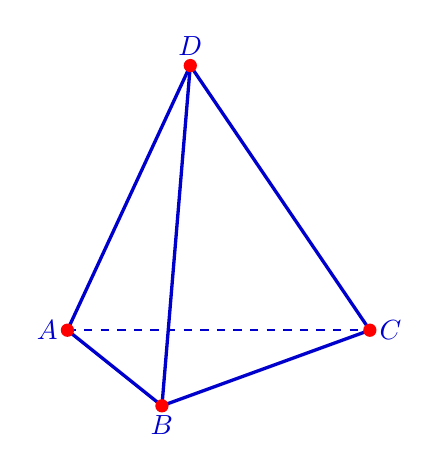
\begin{tikzpicture}[scale=1.2]
    % Định nghĩa tọa độ các đỉnh tứ diện ABCD
    \coordinate (A) at (0, 0);
    \coordinate (B) at (1.0, -0.8);
    \coordinate (C) at (3.2, 0);
    \coordinate (D) at (1.3, 2.8);

    % Đường khuất (nét đứt)
    \draw[thick, dashed, blue!80!black] (A) -- (C);

    % Các cạnh nhìn thấy (nét liền)
    \draw[very thick, blue!80!black] (A) -- (B) -- (C) -- (D) -- cycle;
    \draw[very thick, blue!80!black] (D) -- (B);

    % Vẽ các điểm nút màu đỏ tại các đỉnh A, B, C, D
    \foreach \p in {A, B, C, D} {
        \fill[red] (\p) circle (2pt);
    }

    % Đặt nhãn cho các điểm
    \node[left, blue!80!black] at (A) {$A$};
    \node[below, blue!80!black] at (B) {$B$};
    \node[right, blue!80!black] at (C) {$C$};
    \node[above, blue!80!black] at (D) {$D$};

\end{tikzpicture}
\end{center}
}{
    \textbf{a)} & \(BM = CN = \dfrac{a\sqrt{3}}{2}\)
    & \textcolor{amberorange}{$\bigcirc$} & \textcolor{amberorange}{$\bigcirc$} \\ \hline
    
    \textbf{b)} & \(\vec{CN} = \dfrac{1}{2}\left( \vec{CA} + \vec{CD} \right)\)
    & \textcolor{amberorange}{$\bigcirc$} & \textcolor{amberorange}{$\bigcirc$} \\ \hline
    
    \textbf{c)} & \(\vec{CN} \cdot \vec{BM} = \dfrac{a^2}{8}\)
    & \textcolor{amberorange}{$\bigcirc$} & \textcolor{amberorange}{$\bigcirc$} \\ \hline
    
    \textbf{d)} & \(\cos\alpha = \dfrac{1}{6}\)
    & \textcolor{amberorange}{$\bigcirc$} & \textcolor{amberorange}{$\bigcirc$} \\
}





\end{document}